\section{Graphen von Funktionen}
\begin{LA}
    {Einführungsaufgaben}{}
    \begin{center}
        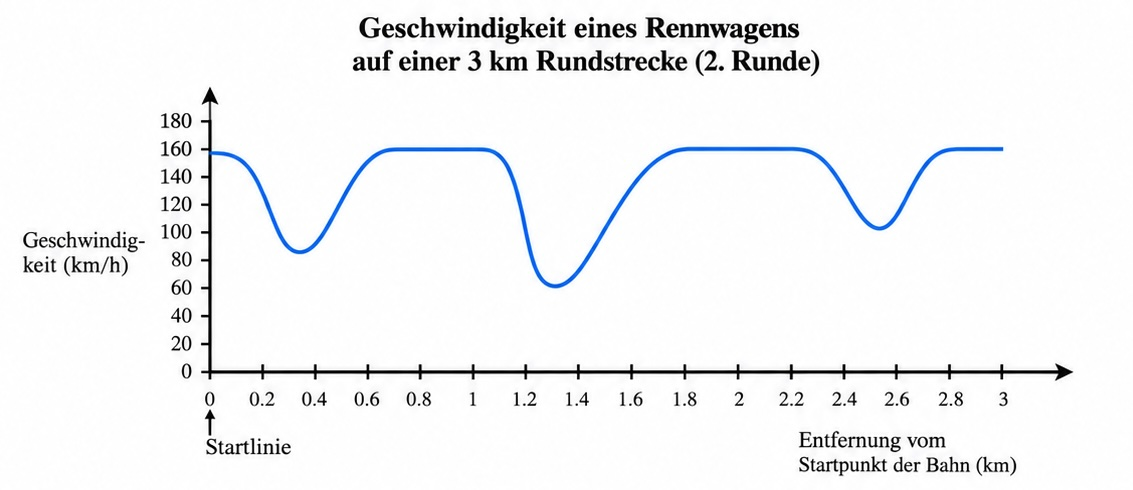
\includegraphics[width = \textwidth]{media/PISA-Graph.jpg}
    \end{center}
    Das Bild oben zeigt den Verlauf der Funktion, die jeder Stelle
    der 3 km langen Rennstrecke die Geschwindigkeit des Rennwagens
    zuordnet.

    \begin{enumerate}
        \item Wo auf der Strecke ist die Geschwindigkeit am niedrigsten?

        \item Was ist die maximale Geschwindigkeit des Rennwagens?

        \item Welche der unten abgebildeten Rennstrecken passt zum
              Geschwindigkeitsprofil oben? Wieso?
    \end{enumerate}
    \begin{center}
        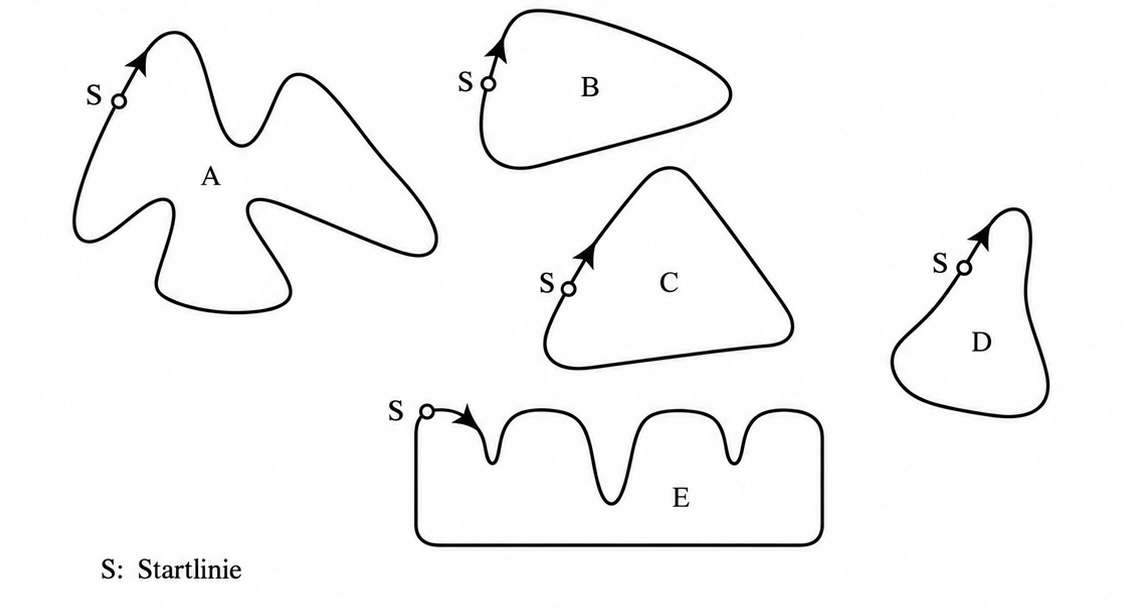
\includegraphics[width = \textwidth]{media/PISA-Strecken.jpg}
    \end{center}
\end{LA}

\clearpage

\subsection*{Das Kartesische Koordinatensystem und der Graph einer Funktion}

Was für zahlreiche Alltagssituationen zutrifft, stimmt auch für Funktionen:
Ein Bild sagt mehr als tausend Worte. Schafft man es, eine Funktion bildlich
darzustellen, so werden ihre Besonderheiten auf einen Blick sichtbar.

Um Funktionen zu visualisieren, verwendet man in der Regel ein
Kartesisches\footnote{Benannt nach René Descartes (1596-1650), französischer Mathematiker und Philosoph auch
    bekannt für \enquote{cogito ergo sum} (Ich denke, also bin ich)} Koordinatensystem:

\begin{center}

    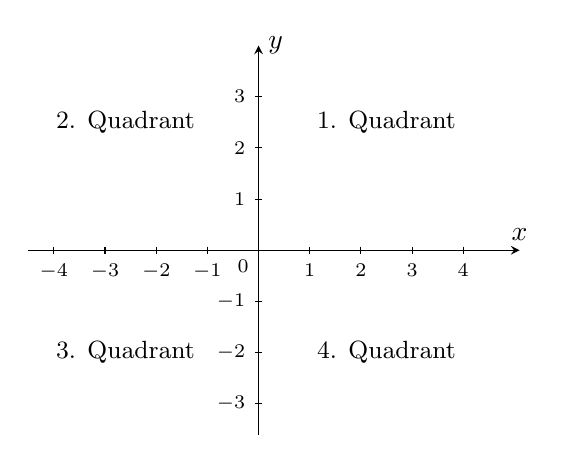
\begin{tikzpicture}[scale=0.65, >=stealth]
        % Koordinatenachsen
        \draw[->, thin] (-4.5,0) -- (5.1,0) node[above] {\(x\)};
        \draw[->, thin] (0,-3.6) -- (0,4.0) node[right] {\(y\)};

        % Skalierung
        \foreach \x in {-4,-3,-2,-1,1,2,3,4} {
                \draw (\x,0.07) -- (\x,-0.07);
                \node[below, font=\scriptsize] at (\x,-0.07) {\(\x\)};
            }
        \foreach \y in {-3,-2,-1,1,2,3} {
                \draw (0.07,\y) -- (-0.07,\y);
                \node[left, font=\scriptsize] at (-0.07,\y) {\(\y\)};
            }
        \node[below left, font=\scriptsize] at (0,0) {\(0\)};

        % Quadranten
        \node[font=\small] at (2.5,2.5) {1. Quadrant};
        \node[font=\small] at (-2.6,2.5) {2. Quadrant};
        \node[font=\small] at (-2.6,-2) {3. Quadrant};
        \node[font=\small] at (2.5,-2) {4. Quadrant};
    \end{tikzpicture}
\end{center}

Ein Kartesisches Koordinatensystem besteht aus zwei zueinander
senkrechten, skalierten Achsen. Die horizontale Achse nennt man
\textbf{\(x\)-Achse} oder \textbf{Abszisse}. Die vertikale
\textbf{\(y\)-Achse} oder \textbf{Ordinate}. Den Schnittpunkt der beiden
Achsen nennt man den \textbf{Ursprung} des Koordinatensystems.
Er wird in der Regel mit \(O\) (für Origo) bezeichnet.

Durch die Achsen wird die Zeichenebene in vier \textbf{Quadranten}
unterteilt, die im Gegenuhrzeigersinn durchnummeriert werden.


Der Graph einer Funktion ist eine Menge von Punkten im
Kartesischen Koordinatensystem:
\begin{center}
    \begin{tikzpicture}[x=0.75cm,y=0.12cm,>=stealth]
        % Achsen
        \draw[->, thin] (-4.4,0) -- (5.8,0) node[above] {\(x\)};
        \draw[->, thin] (0,-26) -- (0,25) node[right] {\(y\)};

        % Skalierung x
        \foreach \x in {-4,-3,-2,-1,1,2,3,4,5} {
                \draw (\x,0.5) -- (\x,-0.5);
                \node[below, font=\scriptsize] at (\x,-0.5) {\(\x\)};
            }

        % Skalierung y
        \foreach \y in {-20,-10,10,20} {
                \draw (0.07,\y) -- (-0.07,\y);
                \node[left, font=\scriptsize] at (-0.07,\y) {\(\y\)};
            }

        \node[below left, font=\scriptsize] at (0,0) {\(0\)};

        % Funktion: f(x) = (1/3)x^3 + x^2
        % f(2) = -16/3 wird durch Vorzeichenwechsel erreicht:
        % f(x) = x^3/3 - 3x^2 + 10x/3
        % Passende Kurve mit Nullstelle und Tiefpunkt bei x=2
        \draw[green!60!black, thick, smooth, domain=-4.3:4.2, samples=150]
        plot (\x,{(\x+3)*\x*(\x-4)/3});

        % Punkt bei x=2
        \fill[blue!70] (2,-6.6666) circle (2pt);

        % Hilfslinien
        \draw[dashed, gray] (2,0) -- (2,-6.6666);
        \draw[dashed, gray] (0,-6.6666) -- (2,-6.6666);

        % Beschriftungen
        %\node[above] at (2,0) {\(2\)};
        \node[left] at (0,-6.6666) {\(-\frac{20}{3}\)};
        \node[below right, blue!70, font=\scriptsize]
        at (2,-6.6666) {\((2,-\frac{20}{3})\)};
        \node[green!60!black] at (-4.2,5) {\(f\)};
    \end{tikzpicture}
\end{center}


Das Bild zeigt den Graphen einer Funktion \(f\).
Der Punkt mit den Koordinaten
\(\left(2\mid-\frac{20}{3}\right)\) liegt auf dem Graphen,
weil die entsprechende Funktion dem Argument \(x=2\)
den Funktionswert \(y=-\frac{20}{3}\) zuordnet, also
\(f(2)=-\frac{20}{3}\).

Am Bild erkennt man auch den Vorteil der grafischen
Darstellung von Funktionen: Anhand des Bildes kann man sofort
sagen, dass im Bereich \(x\in[-4,4]\) der höchste Funktionswert
für \(x\approx -1.8\) erreicht wird und ungefähr \(y\approx 4\) beträgt.

\begin{definition}
    {Graph einer Funktion}{}
    Der Graph einer Funktion \(f\) ist die Menge der Punkte mit den
    Koordinaten \((x, y)\) im Kartesischen Koordinatensystem mit der
    Eigenschaft, dass \(y\) der Output der Funktion zum Input \(x\) ist:

    \[
        \operatorname{Graph} f
        = \{(x, y) \mid y=f(x)\}
    \]
\end{definition}

\subsection*{Nicht jede Kurve ist der Graph einer Funktion}

Im ersten Kapitel wurde eine wichtige Eigenschaft von Funktionen
betont: Die Zuordnung muss \emph{eindeutig} sein. In anderen Worten:
Jedem zulässigen Input wird \emph{genau ein} Output zugeordnet.
Für den Graphen heisst das, dass es keine zwei Graphenpunkte geben
kann mit der gleichen \(x\)-Koordinate.

Anders ausgedrückt: Jede Parallele zur \(y\)-Achse wird immer
höchstens einen Schnittpunkt mit einem Funktionsgraphen haben.

\begin{center}
    \begin{tikzpicture}[scale=0.9, >=stealth]

        % Koordinatenachsen
        \draw[->] (-4.3,0) -- (4.1,0)node[above] {\(x\)};
        \draw[->] (0,-4.1) -- (0,3.1) node[right] {\(y\)};

        % Skalierung x-Achse
        \foreach \x in {-4,-3,-2,-1,1,2,3} {
                \draw (\x,0.05) -- (\x,-0.05);
                \node[below] at (\x,-0.05) {\small \(\x\)};
            }
        \node[below left] at (0,0) {\small \(0\)};

        % Skalierung y-Achse
        \foreach \y in {-4,-3,-2,-1,1,2} {
                \draw (0.05,\y) -- (-0.05,\y);
                \node[left] at (-0.05,\y) {\small \(\y\)};
            }

        % Kurve (parametrisch)
        \draw[green!60!black, thick, smooth,, samples=200,
            domain=-4:1, variable=\t]
        plot ({-2.85 + 0.65*(\t+1.7)^2},
            {\t});

        % Vertikale Testgerade
        \draw[dashed, very thick, gray!75!black]
        (-2, -4.1) -- (-2,3.1);

    \end{tikzpicture}
\end{center}

Die Kurve in der Grafik kann nicht der Graph einer Funktion
sein, weil die Parallele zur \(y\)-Achse an der Stelle \(x=-2\)
die Kurve in zwei Punkten schneidet. Das würde bedeuten, dass die
entsprechende Zuordnung für den Input \(x=-2\) zwei mögliche
Outputs liefert (ungefähr \(-0.5\) und \(-2.9\)). Das widerspricht
der Vorgabe, dass die Funktion eindeutig sein muss.

\subsection*{Von der Funktionsgleichung zum Funktionsgraphen}

Am Beispiel der Funktion \(g(x)=2x-x^2\) soll aufgezeigt werden,
wie man den Graphen einer Funktion zeichnen kann, wenn man die
Funktionsgleichung kennt.

Als Erstes wird eine sogenannte \emph{Wertetabelle} erstellt.
Darin werden die Funktionswerte an einigen Stellen eingetragen.
Für das vorliegende Beispiel wurden die Werte für ganzzahlige
Argumente zwischen \(-3\) und \(5\) berechnet:

\begin{center}
    \renewcommand{\arraystretch}{1.5}
    \begin{tabular}{|c||*{9}{c|}}
        \hline
        \(x\)      & \(-3\)  & \(-2\) & \(-1\) & \(0\) & \(1\) & \(2\) & \(3\)  & \(4\)  & \(5\)   \\
        \hline
        \(y=g(x)\) & \(-15\) & \(-8\) & \(-3\) & \(0\) & \(1\) & \(0\) & \(-3\) & \(-8\) & \(-15\) \\
        \hline
    \end{tabular}
\end{center}

Anhand der Wertetabelle erkennt man, dass für die vorliegende
Funktion ein Koordinatensystem nötig ist, auf welchem die
\(x\)-Achse im Bereich \(-3\) bis \(5\) abgebildet ist,
während die \(y\)-Werte zwischen \(-15\) und \(1\) liegen:

\begin{center}
    \begin{tikzpicture}[
            x=1.2cm,
            y=0.3cm,
            >=stealth
        ]
        % Koordinatenachsen
        \draw[->] (-4.4,0) -- (6.3,0) node[above] {\(x\)};
        \draw[->] (0,-18.5) -- (0,7.2) node[right] {\(y\)};

        % Skalierung x-Achse
        \foreach \x in {-4,-3,-2,-1,1,2,3,4,5,6} {
                \draw (\x,0.15) -- (\x,-0.15);
                \node[below, font=\small] at (\x,-0.15) {\(\x\)};
            }

        % Ursprung
        \node[below left, font=\small] at (0,0) {\(0\)};

        % Skalierung y-Achse
        \foreach \y in {-15,-10,-5,5} {
                \draw (-0.06,\y) -- (0.06,\y);
                \node[left, font=\small] at (-0.06,\y) {\(\y\)};
            }

    \end{tikzpicture}
\end{center}

Jedes Zahlenpärchen \((x, y)\) in der Wertetabelle entspricht
einem Punkt auf dem Graphen:
% Erstes Bild: Punkte der Wertetabelle
\begin{center}
    \begin{tikzpicture}[x=1.2cm, y=0.3cm, >=stealth]

        % Koordinatenachsen
        \draw[->] (-4.4,0) -- (6.3,0) node[above] {\(x\)};
        \draw[->] (0,-18.5) -- (0,7.2) node[right] {\(y\)};

        % Skalierung x-Achse
        \foreach \x in {-4,-3,-2,-1,1,2,3,4,5,6} {
                \draw (\x,0.15) -- (\x,-0.15);
                \node[below, font=\small] at (\x,-0.15) {\(\x\)};
            }
        \node[below left, font=\small] at (0,0) {\(0\)};

        % Skalierung y-Achse
        \foreach \y in {-15,-10,-5,5} {
                \draw (-0.06,\y) -- (0.06,\y);
                \node[left, font=\small] at (-0.06,\y) {\(\y\)};
            }

        % Punkte der Wertetabelle
        \foreach \x/\y in {
                -3/-15,
                -2/-8,
                -1/-3,
                0/0,
                1/1,
                2/0,
                3/-3,
                4/-8,
                5/-15
            } {
                \filldraw[fill=gray!70, draw=black]
                (\x,\y) circle (2.5pt);
            }

    \end{tikzpicture}
\end{center}

Da der Definitionsbereich von \(g\) alle reellen Zahlen umfasst,
ist diese Menge von einzelnen Punkten nur ein kleiner Ausschnitt
des Graphen. Den Verlauf zwischen den Punkten schätzt man,
indem man die Punkte durch eine \enquote{glatte} Kurve verbindet.
Ist man sich unsicher, können auch noch zusätzliche Werte
berechnet werden, wie z.\,B.
\[
    g\left(\frac{1}{2}\right)=\frac{3}{4}.
\]

% Zweites Bild: Punkte und Funktionsgraph
\begin{center}
    \begin{tikzpicture}[x=1.2cm, y=0.3cm, >=stealth]

        % Koordinatenachsen
        \draw[->] (-4.4,0) -- (6.3,0) node[above] {\(x\)};
        \draw[->] (0,-18.5) -- (0,7.2) node[right] {\(y\)};

        % Skalierung x-Achse
        \foreach \x in {-4,-3,-2,-1,1,2,3,4,5,6} {
                \draw (\x,0.15) -- (\x,-0.15);
                \node[below, font=\small] at (\x,-0.15) {\(\x\)};
            }
        \node[below left, font=\small] at (0,0) {\(0\)};

        % Skalierung y-Achse
        \foreach \y in {-15,-10,-5,5} {
                \draw (-0.06,\y) -- (0.06,\y);
                \node[left, font=\small] at (-0.06,\y) {\(\y\)};
            }

        % Funktionsgraph g(x) = 2x - x^2
        \draw[thick, gray!75!black, smooth,
            domain=-3.3:5.3, samples=150]
        plot (\x,{2*\x-\x*\x});

        % Punkte der Wertetabelle
        \foreach \x/\y in {
                -3/-15,
                -2/-8,
                -1/-3,
                0/0,
                1/1,
                2/0,
                3/-3,
                4/-8,
                5/-15,
                0.5/0.75
            } {
                \filldraw[fill=gray!70, draw=black]
                (\x,\y) circle (2.5pt);
            }

        % Beschriftung des Graphen
        \node[below left] at (-3.3,-17.49) {\(g\)};

    \end{tikzpicture}
\end{center}

\clearpage
\begin{ueb}
    {}{}
    \begin{enumerate}
        \item Welche Kurve ist der Graph einer Funktion \(x\mapsto y\)?
              \begin{center}
                  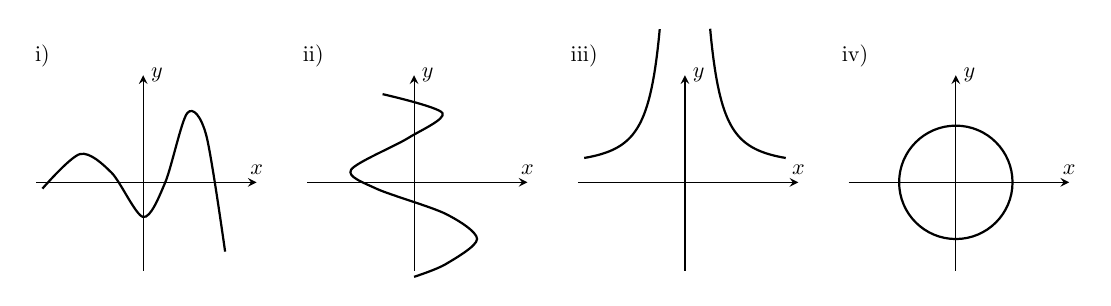
\begin{tikzpicture}[
                          scale=0.8,
                          transform shape,
                          >=stealth,
                          kurve/.style={thick, smooth},
                          achse/.style={->, thin}
                      ]

                      % ==========================================
                      % i) Funktionsgraph
                      % ==========================================
                      \begin{scope}[shift={(0,0)}]
                          \draw[achse] (-1.7,0) -- (1.8,0) node[above] {\(x\)};
                          \draw[achse] (0,-1.4) -- (0,1.7) node[right] {\(y\)};

                          \draw[kurve]
                          plot[smooth] coordinates {
                                  (-1.6,-0.1)
                                  (-1.0,0.45)
                                  (-0.5,0.15)
                                  (0,-0.55)
                                  (0.35,0)
                                  (0.7,1.1)
                                  (1.0,0.75)
                                  (1.3,-1.1)
                              };

                          \node[above] at (-1.6,1.7) {i)};
                      \end{scope}

                      % ==========================================
                      % ii) Keine Funktion
                      % ==========================================
                      \begin{scope}[shift={(4.3,0)}]
                          \draw[achse] (-1.7,0) -- (1.8,0) node[above] {\(x\)};
                          \draw[achse] (0,-1.4) -- (0,1.7) node[right] {\(y\)};

                          \draw[kurve]
                          plot[smooth] coordinates {
                                  (-0.5,1.4)
                                  (0.45,1.1)
                                  (-0.1,0.7)
                                  (-1.0,0.2)
                                  (-0.6,-0.1)
                                  (0.5,-0.5)
                                  (1.0,-0.9)
                                  (0.5,-1.3)
                                  (0,-1.5)
                              };

                          \node[above] at (-1.6,1.7) {ii)};
                      \end{scope}

                      % ==========================================
                      % iii) Funktionsgraph
                      % ==========================================
                      \begin{scope}[shift={(8.6,0)}]
                          \draw[achse] (-1.7,0) -- (1.8,0) node[above] {\(x\)};
                          \draw[achse] (0,-1.4) -- (0,1.7) node[right] {\(y\)};

                          % Zwei Äste einer Funktion
                          \draw[kurve, domain=-1.6:-0.4, samples=100]
                          plot (\x,{0.25+0.35/(\x*\x)});

                          \draw[kurve, domain=0.4:1.6, samples=100]
                          plot (\x,{0.25+0.35/(\x*\x)});

                          \node[above] at (-1.6,1.7) {iii)};
                      \end{scope}

                      % ==========================================
                      % iv) Keine Funktion (Kreis)
                      % ==========================================
                      \begin{scope}[shift={(12.9,0)}]
                          \draw[achse] (-1.7,0) -- (1.8,0) node[above] {\(x\)};
                          \draw[achse] (0,-1.4) -- (0,1.7) node[right] {\(y\)};

                          \draw[kurve] (0,0) circle[radius=0.9cm];

                          \node[above] at (-1.6,1.7) {iv)};
                      \end{scope}

                  \end{tikzpicture}
              \end{center}
        \item Ist die grafisch dargestellte Zuordnung \(x\mapsto y\)
              eine Funktion?
              \begin{center}
                  \begin{tikzpicture}[
                          scale=0.8,
                          >=stealth,
                          kurve/.style={thick, smooth},
                          achse/.style={->, thin}
                      ]

                      % ==========================================
                      % i) Funktionsgraph
                      % ==========================================
                      \begin{scope}[shift={(0,0)}]
                          \draw[achse] (-1.9,0) -- (2.2,0) node[above] {\(x\)};
                          \draw[achse] (0,-0.7) -- (0,2.1) node[right] {\(y\)};

                          \draw[kurve]
                          plot[smooth] coordinates {
                                  (-1.3,2.0)
                                  (-1.15,0.75)
                                  (-0.9,0.3)
                                  (-0.6,0.65)
                                  (-0.2,1.5)
                                  (0,1.65)
                                  (0.3,1.3)
                                  (0.7,0.3)
                                  (0.95,-0.25)
                                  (1.2,-0.1)
                                  (1.45,0.8)
                                  (1.55,2.0)
                              };

                          \node[above] at (-1.9,2.1) {i)};
                      \end{scope}

                      % ==========================================
                      % ii) Einzelne Punkte
                      % ==========================================
                      \begin{scope}[shift={(5.2,0)}]
                          \draw[achse] (-1.4,0) -- (3.6,0) node[right] {\(x\)};
                          \draw[achse] (0,-0.3) -- (0,2.8) node[above] {\(y\)};

                          % Hilfslinien
                          \draw[dotted, gray] (-1,0) -- (-1,2);
                          \draw[dotted, gray] (1,0) -- (1,2);
                          \draw[dotted, gray] (2,0) -- (2,2);
                          \draw[dotted, gray] (3,0) -- (3,2);
                          \draw[dotted, gray] (0,1) -- (2,1);
                          \draw[dotted, gray] (0,2) -- (3,2);

                          % Skalierung
                          \foreach \x in {-1,0,1,2,3} {
                                  \draw (\x,0.05) -- (\x,-0.05);
                                  \node[below] at (\x,-0.05) {\small \(\x\)};
                              }

                          \foreach \y in {1,2} {
                                  \draw (-0.05,\y) -- (0.05,\y);
                                  \node[left] at (-0.05,\y) {\small \(\y\)};
                              }

                          % Punkte
                          \foreach \x/\y in {
                                  -1/0,
                                  0/0,
                                  1/2,
                                  2/1,
                                  3/2
                              } {
                                  \fill (\x,\y) circle (3pt);
                              }

                          \node[above] at (-1.4,2.8) {ii)};
                      \end{scope}

                      % ==========================================
                      % iii) Seitliche Parabel y^2 = x
                      % ==========================================
                      \begin{scope}[shift={(12,0)}]
                          \draw[achse] (-0.5,0) -- (4.2,0) node[above] {\(x\)};
                          \draw[achse] (0,-2.1) -- (0,2.2) node[right] {\(y\)};

                          % Parabel parametrisch
                          \draw[kurve, domain=-1.8:1.8, samples=100,
                              variable=\t]
                          plot ({\t*\t},{\t});

                          \node at (2.8,1.1) {\(y^2=x\)};
                          \node[above] at (-0.5,2.2) {iii)};
                      \end{scope}

                  \end{tikzpicture}
              \end{center}

        \item Liegt der Punkt exakt auf dem Graphen von \(f\)
              mit \(f(x)=\sqrt{2-x}\)?

              \begin{enumerate}
                  \item \(A(0,1.4)\)
                  \item \(B(-2,-2)\)
                  \item \(C(-14,4)\)
              \end{enumerate}

        \item Gegeben ist der Graph einer Funktion
              \(f\colon x\mapsto y=f(x)\).
              Beantworten Sie die folgenden Fragen anhand der
              nebenstehenden Darstellung.

              \begin{enumerate}
                  \item Für welche Argumente \(x\) ist \(f(x)=3\)?
                  \item Für welche Stellen \(x\) ist \(y=0\)?
                  \item Welchen Wert hat \(f(2)\) und welchen Wert hat \(f(5)\)?
              \end{enumerate}

              \begin{center}
                  \begin{tikzpicture}[scale=0.85, >=stealth]

                      % Gitternetz
                      \draw[step=1, gray!50, dotted]
                      (-4,-2) grid (7,5);

                      % Koordinatenachsen
                      \draw[->, thick] (-4,0) -- (8,0) node[right] {\(x\)};
                      \draw[->, thick] (0,-2) -- (0,6) node[above] {\(y\)};

                      % Skalierung x-Achse
                      \foreach \x in {-4,-3,-2,-1,1,2,3,4,5,6,7} {
                              \draw (\x,0.1) -- (\x,-0.1);
                              \node[below] at (\x,-0.1) {\small \(\x\)};
                          }

                      % Skalierung y-Achse
                      \foreach \y in {-2,-1,1,2,3,4,5} {
                              \draw (-0.1,\y) -- (0.1,\y);
                              \node[left] at (-0.1,\y) {\small \(\y\)};
                          }

                      % Funktionsgraph 
                      \draw[thick, smooth,
                          domain=-3.2:7, samples=150]
                      plot (\x,{(\x+3)*(\x-3)*(\x-6)*2/27});





                  \end{tikzpicture}
              \end{center}
        \item Erstellen Sie eine Wertetabelle und zeichnen Sie den Graphen
              der folgenden Funktionen:

              \begin{enumerate}
                  \item \(a(x)=\frac{x}{2}\)
                  \item \(b(x)=-\frac{1}{3}x+6\)
                  \item \(c(x)=2\sqrt{x}\)
                  \item \(d(x)=-3\sqrt{x}\)
                  \item \(e(x)=\frac{5}{x+3}\)
                  \item \(f(x)=\frac{1}{2}x^2-\frac{9}{2}\)
                  \item \(g(x)=\sqrt{2x+7}\)
              \end{enumerate}

        \item Zeichnen Sie die Graphen der folgenden Funktionen.

              \emph{Tipp:} Überlegen Sie, wie sich jeder Graph ab
              Aufgabe b) von dem davor unterscheidet.

              \begin{enumerate}
                  \item \(x\mapsto |x|\)
                  \item \(x\mapsto -|x|\)
                  \item \(x\mapsto -|x|+1\)
                  \item \(x\mapsto \bigl|-|x|+1\bigr|\)
              \end{enumerate}
        \item Welcher Graph gehört zu welcher Funktion?

              \begin{center}
                  \begin{tikzpicture}[
                          x=0.47cm,
                          y=0.47cm,
                          >=stealth,
                          achse/.style={->, thin},
                          kurve/.style={thick},
                          raster/.style={gray!30, thin},
                          scale=0.8
                      ]

                      % Hilfsmakro für Koordinatensysteme
                      % Argumente: x-Verschiebung, y-Verschiebung
                      \newcommand{\koordinatensystem}[2]{
                          \begin{scope}[shift={(#1,#2)}]
                              \draw[achse] (-4.5,0) -- (9,0) node[below] {\(x\)};
                              \draw[achse] (0,-2.5) -- (0,6.8) node[right] {\(y\)};

                              \foreach \x in {-4,-2,2,4,6,8} {
                                      \draw (\x,0.1) -- (\x,-0.1);
                                      \node[below, font=\scriptsize] at (\x,-0.1) {\(\x\)};
                                  }

                              \foreach \y in {-2,2,4,6} {
                                      \draw (0.1,\y) -- (-0.1,\y);
                                      \node[left, font=\scriptsize] at (-0.1,\y) {\(\y\)};
                                  }

                              \node[below left, font=\scriptsize] at (0,0) {\(0\)};
                          \end{scope}
                      }

                      % ==========================================
                      % a) y = x
                      % ==========================================
                      \koordinatensystem{0}{0}

                      \begin{scope}
                          \draw[kurve, domain=-3:6.5, samples=100]
                          plot (\x,\x);
                          \node[font=\large] at (-4.2,7.5) {a)};
                      \end{scope}

                      % ==========================================
                      % b) y = sqrt(x-1)
                      % ==========================================
                      \koordinatensystem{17}{0}

                      \begin{scope}[shift={(17,0)}]
                          \draw[kurve, domain=1:9, samples=100]
                          plot (\x,{sqrt(\x-1)});
                          \node[font=\large] at (-4.2,7.5) {b)};
                      \end{scope}

                      % ==========================================
                      % c) y = -1.2x + 3
                      % ==========================================
                      \koordinatensystem{0}{-13}

                      \begin{scope}[shift={(0,-13)}]
                          \draw[kurve, domain=-2.5:4.3, samples=100]
                          plot (\x,{-1.2*\x+3});
                          \node[font=\large] at (-4.2,7.5) {c)};
                      \end{scope}

                      % ==========================================
                      % d) y = 1.5^x
                      % ==========================================
                      \koordinatensystem{17}{-13}

                      \begin{scope}[shift={(17,-13)}]
                          \draw[kurve, domain=-6:4.5, samples=100]
                          plot (\x,{pow(1.5,\x)});
                          \node[font=\large] at (-4.2,7.5) {d)};
                      \end{scope}

                      % ==========================================
                      % e) y = 0.5x^2 - 1.5x
                      % ==========================================
                      \koordinatensystem{0}{-26}

                      \begin{scope}[shift={(0,-26)}]
                          \draw[kurve, domain=-2.2:5.2, samples=100]
                          plot (\x,{0.5*\x*\x-1.5*\x});
                          \node[font=\large] at (-4.2,7.5) {e)};
                      \end{scope}

                      % ==========================================
                      % f) y = 0.7x - 2
                      % ==========================================
                      \koordinatensystem{17}{-26}

                      \begin{scope}[shift={(17,-26)}]
                          \draw[kurve, domain=-0.5:9, samples=100]
                          plot (\x,{0.7*\x-2});
                          \node[font=\large] at (-4.2,7.5) {f)};
                      \end{scope}

                      % ==========================================
                      % g) y = 2/(x+1)
                      % ==========================================
                      \koordinatensystem{0}{-39}

                      \begin{scope}[shift={(0,-39)}]
                          \draw[kurve, domain=-4.5:-1.3, samples=100]
                          plot (\x,{2/(\x+1)});

                          \draw[kurve, domain=-0.7:9, samples=100]
                          plot (\x,{2/(\x+1)});

                          \node[font=\large] at (-4.2,7.5) {g)};
                      \end{scope}

                      % ==========================================
                      % Funktionsgleichungen
                      % ==========================================
                      \begin{scope}[shift={(17,-39)}]
                          \node[anchor=west, font=\large] at (-4,7)
                          {(i) \quad \(y=0.7x-2\)};

                          \node[anchor=west, font=\large] at (-4,5)
                          {(ii) \quad \(y=-1.2x+3\)};

                          \node[anchor=west, font=\large] at (-4,3)
                          {(iii) \quad \(y=x\)};

                          \node[anchor=west, font=\large] at (-4,1)
                          {(iv) \quad \(y=\dfrac{2}{x+1}\)};

                          \node[anchor=west, font=\large] at (-4,-1)
                          {(v) \quad \(y=0.5x^2-1.5x\)};

                          \node[anchor=west, font=\large] at (-4,-3)
                          {(vi) \quad \(y=1.5^x\)};

                          \node[anchor=west, font=\large] at (-4,-5)
                          {(vii) \quad \(y=\sqrt{x-1}\)};
                      \end{scope}

                  \end{tikzpicture}
              \end{center}
              ```
        \item Zeichnen Sie die Graphen der folgenden Funktionen.

              \begin{enumerate}
                  \item \(y=\operatorname{sgn}(x)\)
                        (Vorzeichenfunktion, siehe \Cref{uebng:funktionsbegriff})

                  \item \(y=\tau(n)\) für
                        \(n\in\{1,2,3,\ldots,10\}\)
                        (Teileranzahl-Funktion, siehe Kapitel \ref{FuGl})
              \end{enumerate}

        \item \textbf{Challenge:}
              \(k\colon x\mapsto\sqrt{9-(x-3)^2}\)

              \begin{enumerate}
                  \item Bestimmen Sie den Definitionsbereich und die Wertemenge
                        von \(k\).

                  \item Erstellen Sie eine Wertetabelle für die zulässigen
                        ganzzahligen Argumente.

                  \item Skizzieren Sie den Graphen von \(k\).

                  \item Um welche spezielle Kurve handelt es sich beim Graphen?

                  \item Beweisen Sie die Vermutung aus d) wie folgt:

                        \begin{enumerate}
                            \item Betrachten Sie einen beliebigen Punkt
                                  \(P=(u, v)\) auf dem Graphen von \(k\).

                            \item Berechnen Sie den Abstand zum Mittelpunkt
                                  mit Pythagoras.

                            \item Formen Sie den Term aus ii) um, bis Sie
                                  das gewünschte Resultat erhalten \dots
                        \end{enumerate}
              \end{enumerate}
    \end{enumerate}
\end{ueb}

\clearpage
\textbf{Lösungen:}
\begin{enumerate}
    \item (i) und (iii).
    \item (i) Ja, (ii) ja, (iii) Nein.
    \item (a) Nein, (b) Nein, (c) Ja.
    \item (a) \(x=-2, x=1, x=7\), (b) \(x=-3, x=0, x=6\), (c) \(f(2)\approx 1.5\), \(f(5)\approx -1.2\).
    \item % Aufgabe 2
          \begin{center}
              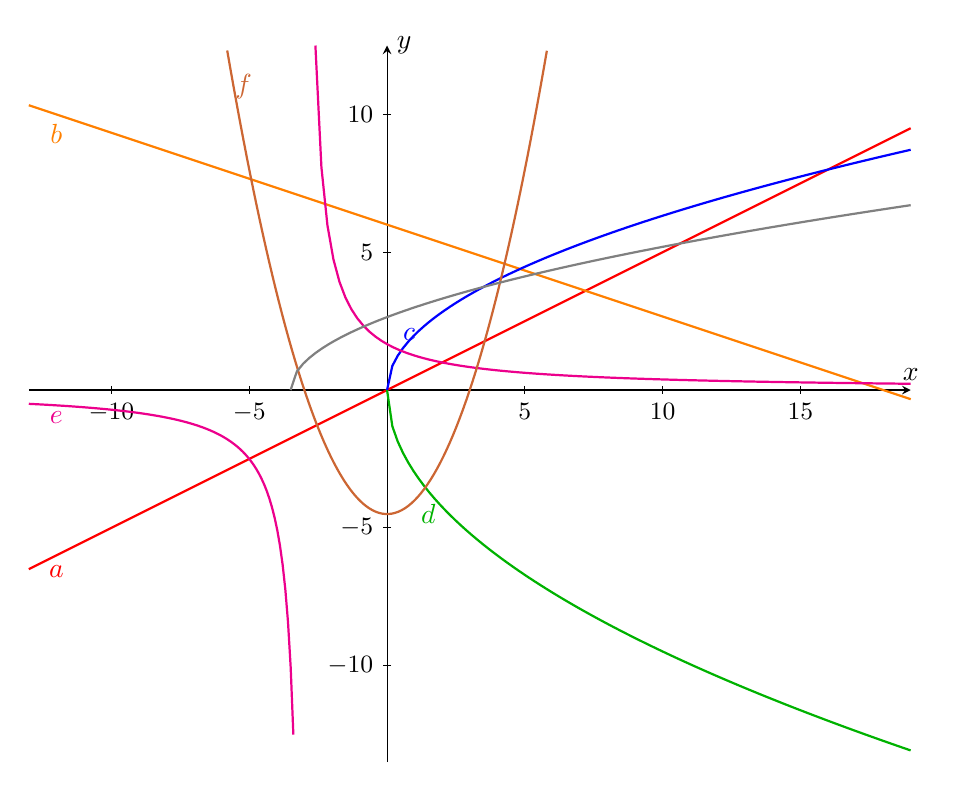
\begin{tikzpicture}[scale=0.35, >=stealth]
                  % Koordinatenachsen
                  \draw[->] (-13,0) -- (19,0) node[above] {\(x\)};
                  \draw[->] (0,-13.5) -- (0,12.5) node[right] {\(y\)};

                  \foreach \x in {-10,-5,5,10,15} {
                          \draw (\x,0.15) -- (\x,-0.15);
                          \node[below] at (\x,-0.15) {\small \(\x\)};
                      }
                  \foreach \y in {-10,-5,5,10} {
                          \draw (0.15,\y) -- (-0.15,\y);
                          \node[left] at (-0.15,\y) {\small \(\y\)};
                      }

                  % a: Gerade
                  \draw[red, thick, domain=-13:19]
                  plot (\x,{0.5*\x});
                  \node[red, below] at (-12,-6) {\(a\)};

                  % b: Fallende Gerade
                  \draw[orange, thick, domain=-13:19]
                  plot (\x,{6-\x/3});
                  \node[orange, below] at (-12,10) {\(b\)};

                  % c: Wurzelfunktion
                  \draw[blue, thick, domain=0:19, samples=100]
                  plot (\x,{2*sqrt(\x)});
                  \node[blue] at (0.8,2) {\(c\)};

                  % d: Negative Wurzelfunktion
                  \draw[green!70!black, thick, domain=0:19, samples=100]
                  plot (\x,{-3*sqrt(\x)});
                  \node[green!70!black] at (1.5,-4.5) {\(d\)};

                  % e: Gebrochenrationale Funktion
                  \draw[magenta, thick, domain=-13:-3.4, samples=100]
                  plot (\x,{5/(\x+3)});
                  \draw[magenta, thick, domain=-2.6:19, samples=100]
                  plot (\x,{5/(\x+3)});
                  \node[magenta] at (-12,-1) {\(e\)};

                  % f: Parabel
                  \draw[brown!80!red, thick, domain=-5.8:5.8, samples=100]
                  plot (\x,{0.5*\x*\x-4.5});
                  \node[brown!80!red] at (-5.2,11) {\(f\)};

                  % g: Wurzelfunktion
                  \draw[gray, thick, domain=-3.5:19, samples=100]
                  plot (\x,{sqrt(2*\x+7)});

              \end{tikzpicture}
          \end{center}

    \item % Aufgabe 3
          Graphen mit Betrag:

          \begin{center}
              \begin{tabular}{|c|c|}
                  \hline
                  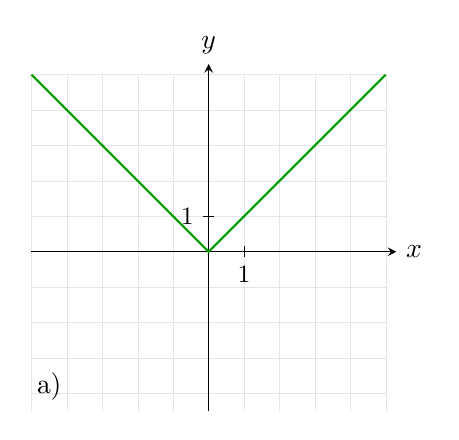
\begin{tikzpicture}[scale=0.45, >=stealth]
                      \draw[step=1, gray!20, very thin] (-5,-4.5) grid (5,5);
                      \draw[->] (-5,0) -- (5.3,0) node[right] {\(x\)};
                      \draw[->] (0,-4.5) -- (0,5.3) node[above] {\(y\)};

                      \foreach \x in {1} {
                              \draw (\x,0.15) -- (\x,-0.15);
                              \node[below] at (\x,-0.15) {\small \(\x\)};
                          }
                      \foreach \y in {1} {
                              \draw (0.15,\y) -- (-0.15,\y);
                              \node[left] at (-0.15,\y) {\small \(\y\)};
                          }


                      \draw[green!60!black, thick, domain=-5:5]
                      plot (\x,{abs(\x)});
                      \node at (-4.5,-3.8) {a)};
                  \end{tikzpicture}
                   &
                  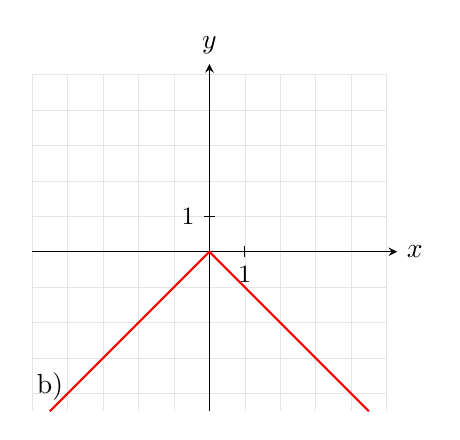
\begin{tikzpicture}[scale=0.45, >=stealth]
                      \draw[step=1, gray!20, very thin] (-5,-4.5) grid (5,5);
                      \draw[->] (-5,0) -- (5.3,0) node[right] {\(x\)};
                      \draw[->] (0,-4.5) -- (0,5.3) node[above] {\(y\)};
                      \foreach \x in {1} {
                              \draw (\x,0.15) -- (\x,-0.15);
                              \node[below] at (\x,-0.15) {\small \(\x\)};
                          }
                      \foreach \y in {1} {
                              \draw (0.15,\y) -- (-0.15,\y);
                              \node[left] at (-0.15,\y) {\small \(\y\)};
                          }
                      \draw[red, thick, domain=-4.5:4.5]
                      plot (\x,{-abs(\x)});
                      \node at (-4.5,-3.8) {b)};
                  \end{tikzpicture}
                  \\ \hline
                  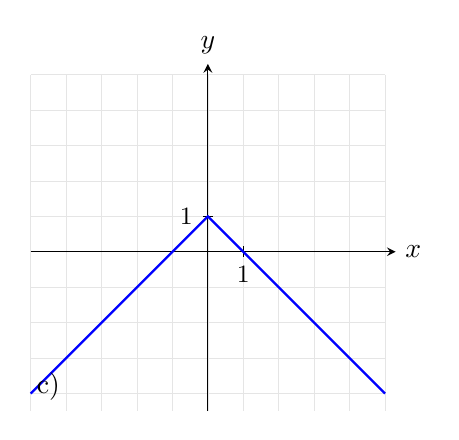
\begin{tikzpicture}[scale=0.45, >=stealth]
                      \draw[step=1, gray!20, very thin] (-5,-4.5) grid (5,5);
                      \draw[->] (-5,0) -- (5.3,0) node[right] {\(x\)};
                      \draw[->] (0,-4.5) -- (0,5.3) node[above] {\(y\)};
                      \foreach \x in {1} {
                              \draw (\x,0.15) -- (\x,-0.15);
                              \node[below] at (\x,-0.15) {\small \(\x\)};
                          }
                      \foreach \y in {1} {
                              \draw (0.15,\y) -- (-0.15,\y);
                              \node[left] at (-0.15,\y) {\small \(\y\)};
                          }
                      \draw[blue, thick, domain=-5:5]
                      plot (\x,{-abs(\x)+1});
                      \node at (-4.5,-3.8) {c)};
                  \end{tikzpicture}
                   &
                  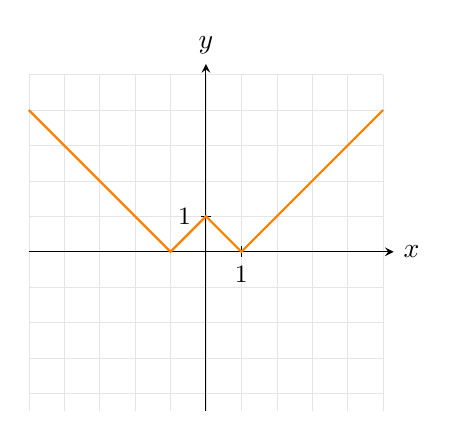
\begin{tikzpicture}[scale=0.45, >=stealth]
                      \draw[step=1, gray!20, very thin] (-5,-4.5) grid (5,5);
                      \draw[->] (-5,0) -- (5.3,0) node[right] {\(x\)};
                      \draw[->] (0,-4.5) -- (0,5.3) node[above] {\(y\)};
                      \foreach \x in {1} {
                              \draw (\x,0.15) -- (\x,-0.15);
                              \node[below] at (\x,-0.15) {\small \(\x\)};
                          }
                      \foreach \y in {1} {
                              \draw (0.15,\y) -- (-0.15,\y);
                              \node[left] at (-0.15,\y) {\small \(\y\)};
                          }
                      \draw[orange, thick]
                      (-5,4) -- (-1,0) -- (0,1) -- (1,0) -- (5,4);
                  \end{tikzpicture}
                  \\ \hline
              \end{tabular}
          \end{center}

    \item
          \begin{enumerate}
              \item a) \(\leftrightarrow\) iii)
              \item b) \(\leftrightarrow\) vii)
              \item c) \(\leftrightarrow\) ii)
              \item d) \(\leftrightarrow\) vi)
              \item e) \(\leftrightarrow\) v)
              \item f) \(\leftrightarrow\) i)
              \item g) \(\leftrightarrow\) iv)
          \end{enumerate}

    \item Graphen spezieller Funktionen:
          \begin{center}
              \begin{tabular}{|c|c|}
                  \hline
                  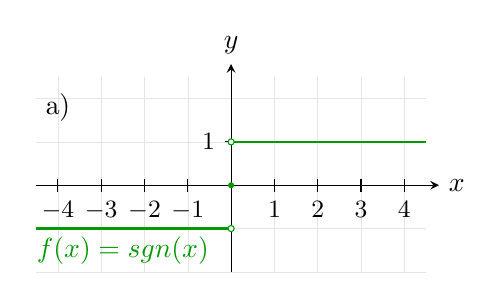
\begin{tikzpicture}[scale=0.55, >=stealth]
                      \draw[step=1, gray!20, very thin] (-4.5,-2) grid (4.5,2.5);
                      \draw[->] (-4.5,0) -- (4.8,0) node[right] {\(x\)};
                      \draw[->] (0,-2) -- (0,2.8) node[above] {\(y\)};

                      \foreach \x in {-4,-3,-2,-1,1,2,3,4} {
                              \draw (\x,0.15) -- (\x,-0.15);
                              \node[below] at (\x,-0.15) {\small \(\x\)};
                          }
                      \foreach \y in {1} {
                              \draw (0.15,\y) -- (-0.15,\y);
                              \node[left] at (-0.15,\y) {\small \(\y\)};
                          }

                      \draw[green!60!black, thick] (-4.5,-1) -- (0,-1);
                      \draw[green!60!black, thick] (0,1) -- (4.5,1);

                      \draw[green!60!black, fill=white] (0,-1) circle (2pt);
                      \draw[green!60!black, fill=white] (0,1) circle (2pt);
                      \fill[green!60!black] (0,0) circle (2pt);

                      \node[green!60!black] at (-2.5,-1.5)
                      {\(f(x)=\operatorname{sgn}(x)\)};
                      \node at (-4,1.8) {a)};
                  \end{tikzpicture}
                   &
                  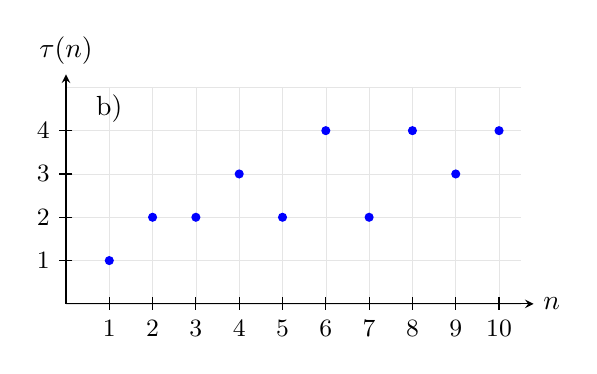
\begin{tikzpicture}[scale=0.55, >=stealth]
                      \draw[step=1, gray!20, very thin] (0,0) grid (10.5,5);
                      \draw[->] (0,0) -- (10.8,0) node[right] {\(n\)};
                      \draw[->] (0,0) -- (0,5.3) node[above] {\(\tau(n)\)};

                      \foreach \x in {1, 2, 3, 4, 5, 6, 7, 8, 9, 10} {
                              \draw (\x,0.15) -- (\x,-0.15);
                              \node[below] at (\x,-0.15) {\small \(\x\)};
                          }
                      \foreach \y in {1,2,3,4} {
                              \draw (0.15,\y) -- (-0.15,\y);
                              \node[left] at (-0.15,\y) {\small \(\y\)};
                          }

                      \foreach \x/\y in {
                              1/1,2/2,3/2,4/3,5/2,
                              6/4,7/2,8/4,9/3,10/4
                          } {
                              \fill[blue] (\x,\y) circle (3pt);
                          }

                      \node at (1,4.5) {b)};
                  \end{tikzpicture}
                  \\ \hline
              \end{tabular}
          \end{center}

    \item \textbf{Challenge:}

          \begin{enumerate}
              \item
                    \(\mathbb{D}=[0,6]\), \(\mathbb{W}=[0,3]\)

              \item Wertetabelle:

                    \begin{center}
                        \renewcommand{\arraystretch}{1.8}
                        \begin{tabular}{|c||c|c|c|c|c|c|c|}
                            \hline
                            \(x\)    & 0 & 1            & 2            & 3 & 4 & 5 & 6 \\ \hline
                            \(k(x)\) & 0 & \(\sqrt{5}\) & \(\sqrt{8}\)
                                     & 3 & \(\sqrt{8}\) & \(\sqrt{5}\) & 0             \\ \hline
                        \end{tabular}
                    \end{center}

              \item Graph:

                    \begin{center}
                        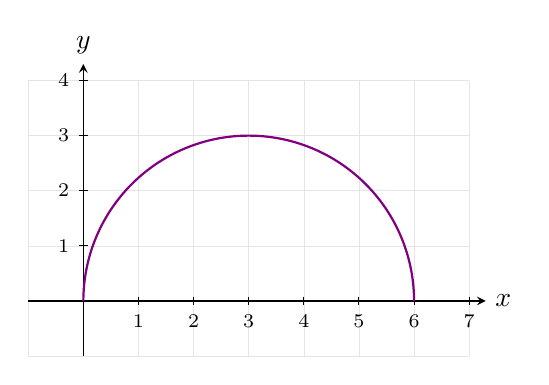
\begin{tikzpicture}[scale=0.7, >=stealth]
                            \draw[step=1, gray!20, very thin]
                            (-1,-1) grid (7,4);

                            \draw[->] (-1,0) -- (7.3,0)
                            node[right] {\(x\)};
                            \draw[->] (0,-1) -- (0,4.3)
                            node[above] {\(y\)};

                            \foreach \x in {1,...,7}
                            \draw (\x,0.08) -- (\x,-0.08)
                            node[below] {\scriptsize \x};

                            \foreach \y in {1,...,4}
                            \draw (0.08,\y) -- (-0.08,\y)
                            node[left] {\scriptsize \y};

                            \draw[violet, thick, samples=200,
                                domain=0:180, smooth]
                            plot ({3+3*cos(\x)},{3*sin(\x)});
                        \end{tikzpicture}
                    \end{center}

              \item Der Graph ist ein Halbkreis mit Mittelpunkt
                    \(M=(3, 0)\) und Radius \(r=3\).

              \item Sei \(P=(u, v)\) ein beliebiger Punkt auf
                    dem Graphen von \(k\).

                    Der Abstand von \(P\) zum Mittelpunkt \(M=(3, 0)\)
                    beträgt nach Pythagoras:

                    \[
                        d=\sqrt{(u-3)^2+v^2}
                    \]

                    Da \(P\) auf dem Graphen von \(k\) liegt, gilt
                    \(v=\sqrt{9-(u-3)^2}\). Somit folgt:

                    \begin{align*}
                        d & = \sqrt{(u-3)^2+
                                  \left(\sqrt{9-(u-3)^2}\right)^2} \\
                          & = \sqrt{(u-3)^2+9-(u-3)^2}             \\
                          & = \sqrt{9}=3
                    \end{align*}

                    Alle Punkte des Graphen von \(k\) haben also
                    den Abstand \(3\) zum Mittelpunkt \(M\).

                    Da ausserdem \(k(x)\geq 0\) gilt,
                    handelt es sich um den oberen Halbkreis.
          \end{enumerate}
\end{enumerate}